\section{Methodology}
We treat each consumer-item as an individual object and generate weekly time series based on historical transaction for 
each object. The target value at each time step (week) takes a binary input, 1/0 (purchased/not purchased).
We adopted walk forward Validation strategy for model testing and generalization. We split the data into 4 parts
based on the time series as shown in Table 1.
We then generate various types of features including datetime related, label encoded and target encoded 
within and across objects. Below are the feature groups we experimented with explicitly or unexplicitly:
\begin{itemize}
\item {\bf Datetime:} Transactional metrics at various temporal cuts including week, month and quarter. 
Datetime related features capturing seasonality and trend.
\item {\bf Consumer-Item Profile:} Transactional metrics at different granularities including consumer, item,
consumer-item, department, aisle, etc. The metrics includes some of likes Time since first order, 
Time since last order, time gap between orders, Reorder rates, Reorder frequency, 
Streak - user purchased the item in a row, Average position in the cart, Total number of orders.
\item {\bf Consumer-Item-Time Profile:} Transactional metrics at the intersection of consumer, item and time.
Interactions capturing consumer behaviour towards items for the given time period.
\end{itemize}
The model we needed to build, thus, should learn to identify similarly behaving time series across latent
parameters, and take into account consumer and item variations in comparing the time series. A row in time series 
is represented by
  \begin{equation}
    \begin{array}{l}
      y\textsubscript{cit}  = f(i\textsubscript{t}, c\textsubscript{t},..,c\textsubscript{t-n}, ic\textsubscript{t}
      ,..,ic\textsubscript{t-n}, d\textsubscript{t},..,d\textsubscript{t-n})
    \end{array}
    \label{eqn:fx}
  \end{equation}
where y\textsubscript{cit} is purchase prediction for consumer 'c' item ’i’ at time ’t’. 
i\textsubscript{t} is attribute of the item ’i’ like category, department, brand, color, size, etc. 
c\textsubscript{t} is attribute of the consumer 'c' like age, sex and transactional attributes. 
ic\textsubscript{t} is transactional attributes of the consumer 'c'  towards item 'i'. 
d\textsubscript{t} is derived from datetime to capture trend and seasonality. 
Finally, n is the number of time lags.
\begin{table}[t]
\caption{Modelling data splits}
\vspace{0.1 in}
\centering
\resizebox{3.3in}{!}
{%
\begin{tabular}{|c|c|c|c|}
\hline
{\bf Data Split} & {\bf Specifications} & {\bf Consumer-Item combinations} & {\bf Max Time-Series length} \\  
\hline\hline
Train  		&  Model training &  5,872 &  46 weeks \\ \hline
Validation	  		&  Hyper-Parameter Optimization &  5,888 &  2 weeks \\ \hline
Test1  		&  Stacked Generalization, F\textsubscript{1}-Maximization & 5,899 &  2 weeks\\ \hline
Test2	  		&  Reporting Accuracy Metrics & 5,910 &  2 weeks\\
\hline
\end{tabular}
}
\label{tab:mlmodels}
\end{table}
\subsection{Loss Function}
Since we are solving Binary classification problem, Binary Cross-Entropy/Log Loss seemed most logical loss function 
for training all our models.
  \begin{equation}
      \begin{array}{l}
        H\textsubscript{p} = - \frac{1}{N}$$\sum_{i=1}^{N}y\textsubscript{i}.log(p(y\textsubscript{i}))+
        (1- y\textsubscript{i}).log(1-p(y\textsubscript{i}))
      \end{array}
    \label{eqn:logloss}
  \end{equation}
where H\textsubscript{p} is total loss and y\textsubscript{i} is the label and p(y\textsubscript{i}) is the predicted probability.
\subsection{Model Architectures}
As mentioned in previous section, traditional machine learning models are not suitable choice for solving Equation~\ref{eqn:fx}. 
Hence, we work with machine learning tree based models like Random Forest Gradient Boosted Trees 
to Deep learning models ranging from Multi Layer Perceptron (MLP), Long Short 
Term Memory (LSTM) and Temporal Convolutional Network (TCN). Architectures of MLP, LSTM, TCN and TCN-LSTM 
models are shown in Figure~\ref{fig:MLP}, Figure~\ref{fig:LSTM}, Figure~\ref{fig:TCN}
and Figure~\ref{fig:TCN-LSTM}. As described in architecture diagrams, data was classified into following groups:
\begin{itemize}
\item {\bf Static Categorical:} These are categorical features which donot vary with time. This includes the consumer
attributes like sex, marital status and location, different item attributes like category, department and brand.
\item {\bf Temporal Categorical:} These are categorical features which vary with time. It includes all the datetime 
related features like week, month of year, etc.
\item {\bf Static Continuous:} These features are static but Continuous. This includes certain consumer attributes like
age and weight, item attributes like size and certain derived features like target encoded features.
\item {\bf Temporal Continuous:} These are time varying Continuous features. All consumer and item related
traditional attributes like number of orders, add to cart order, etc. falls under this class.
\end{itemize}
In all the above neural network architectures, we learn the embeddings of the categorical features during training phase.
We embed these attributes in order to both compress their representations while preserving
salient features, as well as capture mutual similarities and differences.
  \begin{figure}[t]
    \centering 
    \caption{Data classification for DNN Architectures} 
    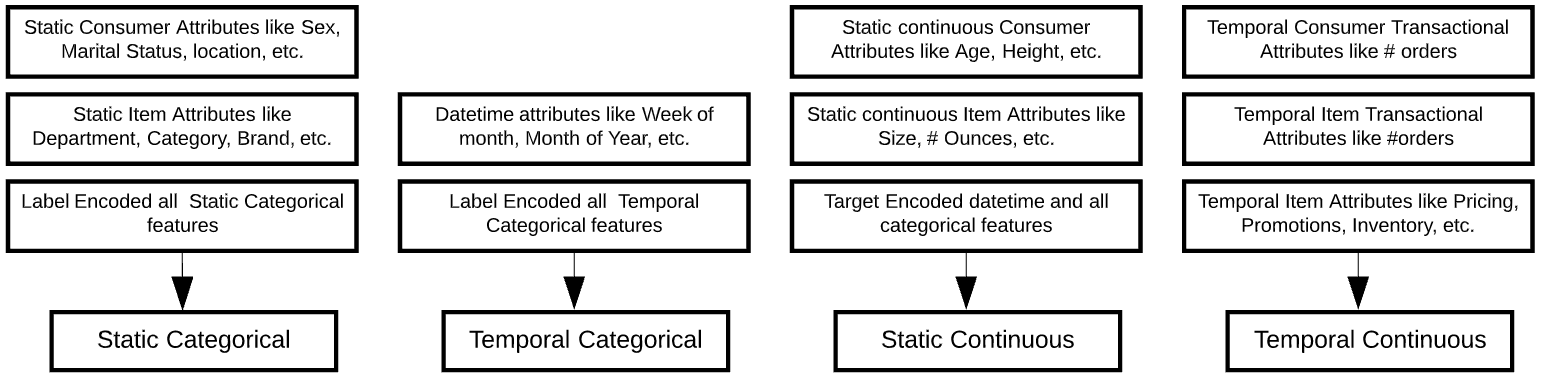
\includegraphics[width=3.3in]{img/dnndata.png} 
    \label{fig:dnndata} 
  \end{figure}
  \begin{figure}[t]
    \centering 
    \caption{Multi Layer Perceptron (MLP)} 
    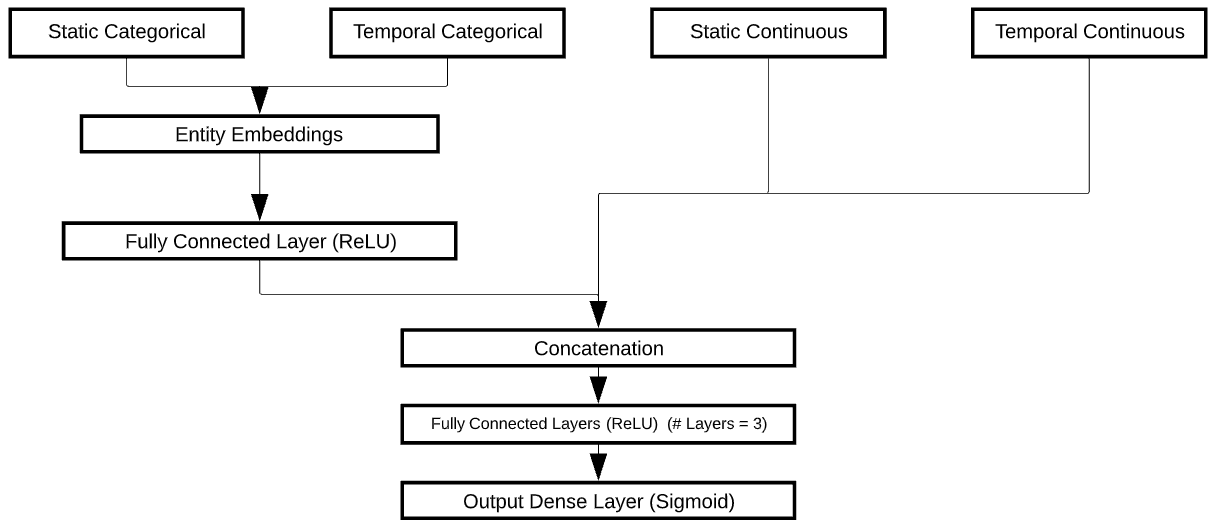
\includegraphics[width=3.3in]{img/MLP.png} 
    \label{fig:MLP} 
  \end{figure}
  \begin{figure}[t]
    \centering 
    \caption{Long Short Term Memory (LSTM)} 
    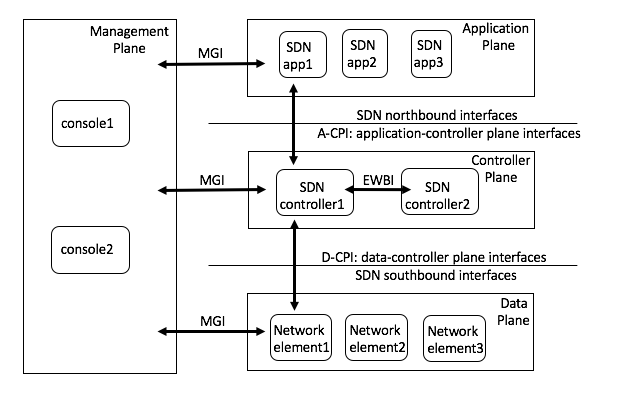
\includegraphics[width=3.3in]{img/LSTM.png} 
    \label{fig:LSTM} 
  \end{figure}
  \begin{figure}[t]
    \centering 
    \caption{Temporal Convolutional Network (TCN)} 
    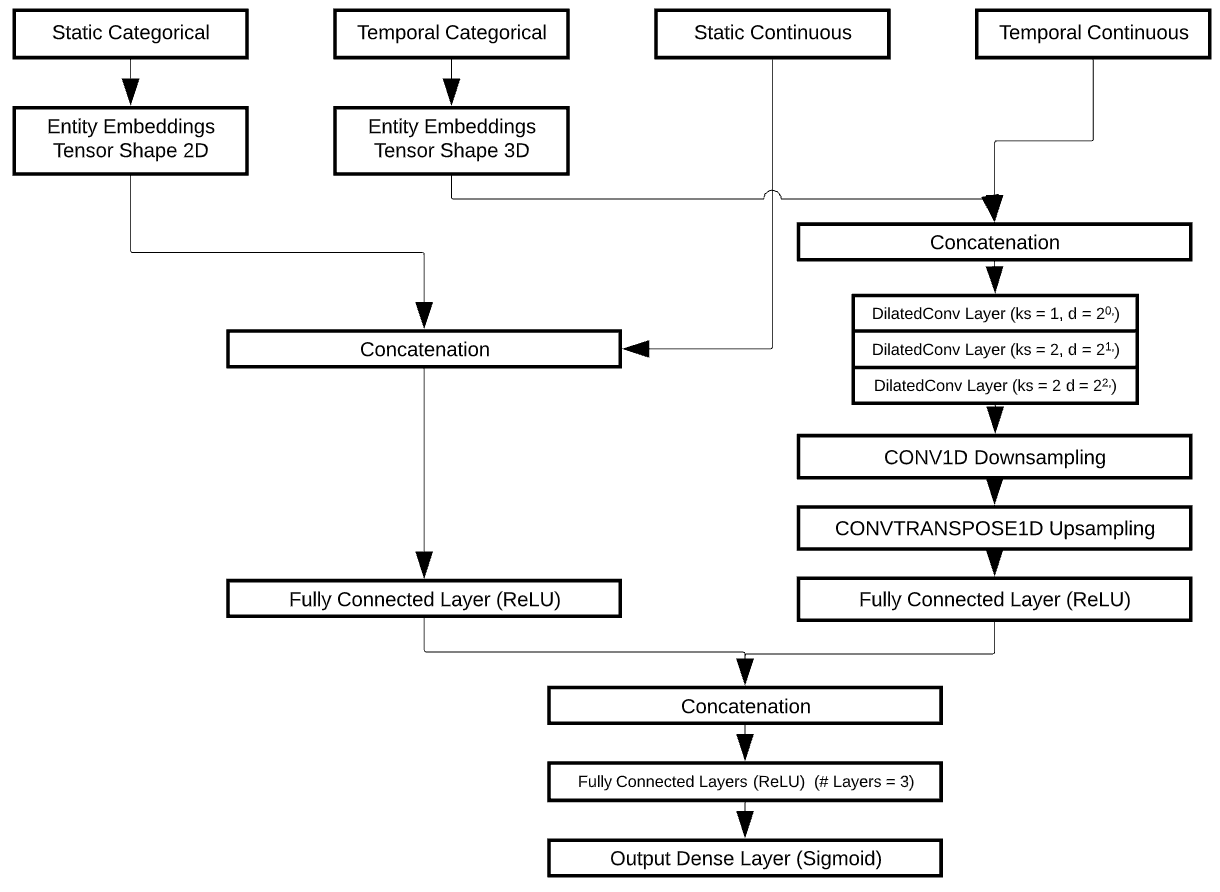
\includegraphics[width=3.3in]{img/TCN.png} 
    \label{fig:TCN} 
  \end{figure}
  \begin{figure}[t]
    \centering 
    \caption{TCN-LSTM} 
    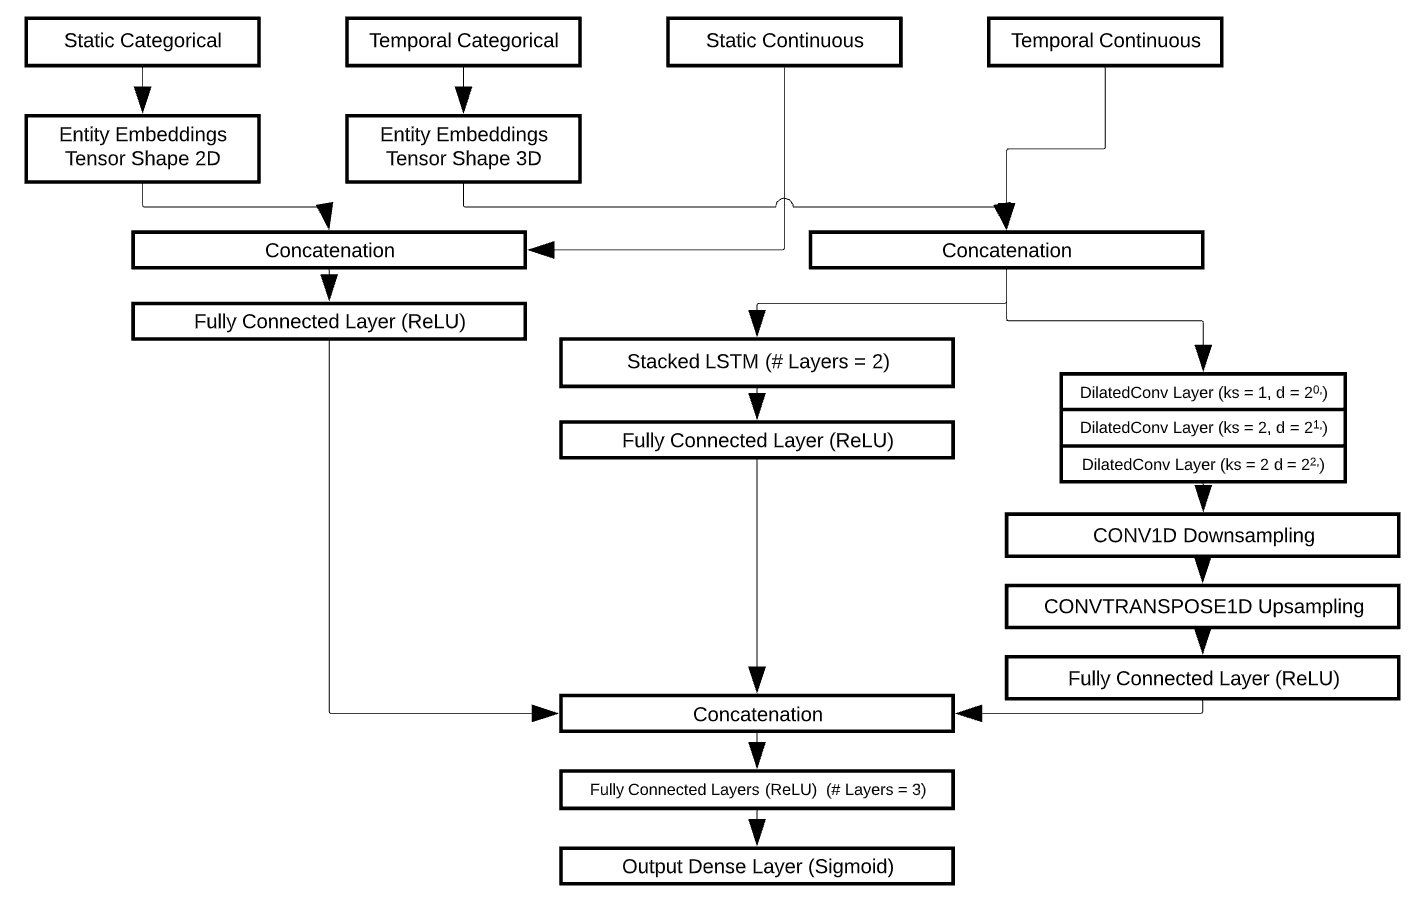
\includegraphics[width=3.3in]{img/TCNLSTM.png} 
    \label{fig:TCNLSTM} 
  \end{figure}
The consumer purchase pattern has huge variation in terms of time of purchase (weekday/weekends), 
cadence of purchase (days to months), purchased item types (dairy/meat/grocery/apparels/etc.)
and brand loyalty (tendency to substitute items). Given such huge variance it becomes imperative 
to cross learn consumer behaviour from like consumer groups. To learn such relationships its very 
important to capture non-linear relationship between target and regressors at the most granular level.
Tree based and Deep learning models are chosen for their ability to model feature interactions even if transient in time, 
so that they capture non-linearity well. Utility of traditional machine learning algorithms like Logistic regression
, SVM and recommender systems are limited given the scale of large retail firms 
(Millions of customers with thousands of products). Such models do not scale well for large sets of data and hyperparameters.

Tree based models and MLP are trained in such a way where lagged values of time varying features are used
to capture temporal dependencies. We use lagged values of temporal features up to last n time steps (n goes till 52 weeks).
Multiple Lagged values as well as Statistical rolling operations like mean, median, quantiles, variance, kurtosis and 
skewness over varying lag periods are used for feature generation. Details around datasets and derived features are explained 
in the following section. This was decided after some preliminary experiments. Hyper-parameters of tree based models are optimized
using Bayesian Hyper-parameter Optimization Technique. LSTM, TCN and TCN-LSTM models were trained in sequence to sequence 
fashion using entire life-cycle data of a time series (Consumer-Item).

We applied empirical approach to tune the hyperparameters for Deep learning models. All hyperparameter Optimization
was performed over Validation dataset. We list some of the params along with the values we used for Deep learning models.
  \begin{itemize}
    \item {\bf Optimizer Parameters:} RMSProp and Adam were used as different trial configurations. The learning rate 
    was experimentally tuned to 1e-3. We also did weight decay of 1e-5 which helped a bit in model Regularization.
    \item {\bf Scheduler Parameters:} Cyclic and ReduceLROnPlateau Learning rates were used as different trial configurations.
    we used 1e-3 as max lr and 1e-6 as base lr for Cyclical learning rate along with the step size being the function of
    length of train loader. ReduceLROnPlateau was tuned for 1e-6 as min lr.
    \item {\bf SWA:} Stochastic Weight Averaging (SWA) is used to improve generalization across Deep Learning
    models. SWA performs an equal average of the weights traversed by SGD with a modified learning rate schedule. We used 
    1e-3 as SWA learning rate.
    \item {\bf Parameter Average:} This applies weighted average over the parameter weights of n best performing epochs 
    (local minimas) from state dictionary post completion of training.
  \end{itemize}
Apart from the above parameters we also iterated enough to tune network parameters like number of epochs, batch size, 
number of Fully Connected Layers, number of LSTM layers, convnet parameters (kernel size, dilations, padding)
and embedding sizes for the categorical features. Binary Cross-Entropy/Log Loss [~\ref{eqn:logloss}] was used as loss 
function for all the models. 
We used Bayesian Optimization Technique for hyper configuration tuning with 100 trials.
Some of the hyperparameters we used for Machine learning models are :
  \begin{itemize}
    \item {\bf Learning Rate:} LR range was set to vary between 1e-3 to 0.5. 
    \item {\bf Max Depth:} Depth range was set between 2 to 12 at the step of 1.
  \end{itemize}
Apart from these, Regularization parameters like Reg Lambda, Min Sample Leaf was also tuned from Bayesian framework.

Deep learning models are built using deep learning framework
PyTorch, and are trained on GCP instance containing 6 CPUs and a single GPU. scikit-learn is used for Tree
based models like RandomForest and Xgboost. We built a total of 60 models, 12 different param configurations for each of 4 
Deep Learning models and 6 best trials for each of 2 Machine Learning models as shown in table 1.
\begin{center}
\begin{table*}[!t]
\caption{Model Specifications}
\centering
\resizebox{\textwidth}{!}{\begin{tabular}{|r|l|r|r|}
  \hline
 {\bf Model Type} & {\bf Trials} & {\bf Model Hyper-Parameters} & {\bf Loss Functions}\\ 
 \hline\hline
MLP	  		&  12 & Optimizer, Scheduler, SWA, Parameter Averaging, Feature Groups, FC Layers & BCELoss\\ \hline
LSTM  		& 12 & Optimizer, Scheduler, SWA, Parameter Averaging, Feature Groups, FC Layers, LSTM Layers & BCELoss \\ \hline
TCN			& 12	& Optimizer, Scheduler, SWA, Parameter Averaging, Feature Groups, FC Layers, Convolution Parameters  & BCELoss\\ \hline
TCN-LSTM 		& 12	& Optimizer, Scheduler, SWA, Parameter Averaging, Feature Groups, FC Layers, LSTM, Convolution Parameters  & BCELoss\\ \hline
Xgboost 		& 6	& Learning rate, Tree Depth, Regularization parameters  & BCELoss\\ \hline
RandomForest 		& 6	& Tree Depth, Evaluation Metrics, Regularization parameters &  BCELoss\\
   \hline
\end{tabular}}
\end{table*} 
\end{center}
\subsection{Stacked Generalization}
For simplicity and better generalization we adopted non-parameteric approach for stacking.
We used Weighted K-Best and K-Best as Stacked Generalization Ensemble model for combining the 60 models (candidates) from Table 1. 
Test1 BCELoss was used as metric to compute weight for each of the 60 candidates. We set k to 5, 10 and 25 and selected 
these top candidates based upon the experiments performed over test1 metrics. Finally, we took Weighted Average of 
the probabilities for Train, Validation, Test1 and Test2 time steps for each consumer-item combination.
\subsection{F1-Maximization}
Post generation of the consumer-item probabilities, we optimize for the purchase cut-off probability based on 
probability distribution of test1 at consumer level. For instance, lets say we generated purchase probabilities for 
n\textsubscript{i} items of b\textsubscript{i} actually purchased items for consumer c\textsubscript{i}.
Let Actual items purchased by consumer c\textsubscript{i} at test1 time step be [Ia\textsubscript{1}, Ia\textsubscript{2}
,.., Ia\textsubscript{b\textsubscript{i}}] whereas items for which the model generated probabilities for the 
consumer c\textsubscript{i} at test1 time step be [Ip\textsubscript{1}, Ip\textsubscript{2} ,.., 
Ip\textsubscript{n\textsubscript{i}}]. 
  \begin{equation}
    \begin{array}{l}
      A\textsubscript{c\textsubscript{i}} = [a\textsubscript{1}, a\textsubscript{2}, .., a\textsubscript{n\textsubscript{i}}] 
       \; \forall \; a\textsubscript{j} \in \; $\{0,1\}$
    \end{array}
    \label{eqn:A}
  \end{equation}
  \begin{equation}
    \begin{array}{l}
      P\textsubscript{c\textsubscript{i}} = [p\textsubscript{1}, p\textsubscript{2}, .., p\textsubscript{n\textsubscript{i}}]
      \; \forall \; p\textsubscript{j} \in \; [0,1]
    \end{array}
    \label{eqn:P}
  \end{equation}
A\textsubscript{c\textsubscript{i}} represents the actuals for consumer c\textsubscript{i}, with a\textsubscript{j} being 1/0 
(purchased/non purchased). P\textsubscript{c\textsubscript{i}} represents the predicted probabilities 
for consumer c\textsubscript{i} for respective item, with p\textsubscript{j} being probability value. 
As mentioned above n\textsubscript{i} is the total items model generated purchase probabilities for.
  \begin{equation}
    \begin{array}{l}
      D(Pr\textsubscript{c\textsubscript{i}}) : P\textsubscript{c\textsubscript{i}}\textsuperscript{1 x n\textsubscript{i}}
      \to P\textsuperscript{'}\textsubscript{c\textsubscript{i}}\textsuperscript{1 x n\textsubscript{i}}
      \;\;  p\textsuperscript{'}\textsubscript{j} = $\{1 if p\textsubscript{j} $\geq$ Pr\textsubscript{c\textsubscript{i}}\}$
    \end{array}
    \label{eqn:Decision}
  \end{equation}
  \begin{equation}
    \begin{array}{l}
      P\textsuperscript{'}\textsubscript{c\textsubscript{i}} = [p\textsuperscript{'}\textsubscript{1}, 
      p\textsuperscript{'}\textsubscript{2}, .., p\textsuperscript{'}\textsubscript{n\textsubscript{i}}]\; 
      \forall \; p\textsuperscript{'}\textsubscript{j} \in \; $\{0,1\}$
    \end{array}
    \label{eqn:Pdash}
  \end{equation}
  \begin{equation}
    \begin{array}{l}
      k\textsubscript{i} =\sum_{i=1}^{n\textsubscript{i}}p\textsuperscript{'}\textsubscript{i}
    \end{array}
    \label{eqn:Pdash}
  \end{equation}
Pr\textsubscript{c\textsubscript{i}} is the probability cut-off.
Decision rule D converts probabilities P\textsubscript{c\textsubscript{i}} to binary predictions 
P\textsuperscript{'}\textsubscript{c\textsubscript{i}} such that if p\textsubscript{j} is less than 
Pr\textsubscript{c\textsubscript{i}} then p\textsuperscript{'}\textsubscript{j} equals 0 else 1. 
k\textsubscript{i} is the total number of predictions which Decision rule D converted to 1 or in other words
number of predictions which model predicted as purchase.
  \begin{equation}
    \begin{array}{l}
      V\textsubscript{Pr\textsubscript{c\textsubscript{i}}} = 
      P\textsuperscript{'}\textsubscript{c\textsubscript{i}}
      \;\times\; A\textsubscript{c\textsubscript{i}}\textsuperscript{T}
      \;
      \Rightarrow	
      \left( \begin{array}{ccc}
      p\textsuperscript{'}\textsubscript{1} & .. & 
      p\textsuperscript{'}\textsubscript{n\textsubscript{i}}
      \end{array} \right)
      \times
      %
      \left( \begin{array}{ccc}
      a\textsubscript{1} \\
      .. \\
      a\textsubscript{n\textsubscript{i}} \\
      \end{array} \right)
    \end{array}
    \label{eqn:probability}
  \end{equation}
V\textsubscript{Pr\textsubscript{c\textsubscript{i}}} represents the number of items with purchase 
probabilities greater than Pr\textsubscript{c\textsubscript{i}} which were actually purchased. Now using the below 
formulae we calculate Precision, Recall and F\textsubscript{1}-score for consumer c\textsubscript{i}.
  \begin{equation}
    \begin{array}{l}
      Precision\textsubscript{c\textsubscript{i}}= \frac{V\textsubscript{Pr\textsubscript{c\textsubscript{i}}}} {k\textsubscript{i}}
      \;\;\;\;\;and\;\;\;\;
      Recall\textsubscript{c\textsubscript{i}}= \frac{V\textsubscript{Pr\textsubscript{c\textsubscript{i}}}} {b\textsubscript{i}}
    \end{array}
    \label{eqn:F1}
  \end{equation}
  \begin{equation}
    \begin{array}{l}
      F\textsubscript{1\textsubscript{c\textsubscript{i}}} = \frac{2 \times Precision\textsubscript{c\textsubscript{i}} 
      \times Recall\textsubscript{c\textsubscript{i}}} 
      {Precision\textsubscript{c\textsubscript{i}} + Recall\textsubscript{c\textsubscript{i}}}
      \;
      \;\;\;\;\Rightarrow	\;\;\;\;
      2 * 
      \frac{
        V\textsubscript{Pr\textsubscript{c\textsubscript{i}}}
      }
      {
        k\textsubscript{i} + b\textsubscript{i}
      }
    \end{array}
    \label{eqn:Optimizer}
  \end{equation}
F\textsubscript{1\textsubscript{c\textsubscript{i}}} becomes the value to be maximised
by finding optimal Pr\textsubscript{c\textsubscript{i}} for consumer c\textsubscript{i}.
We apply the above Optimization function over test1 probability distribution 
at a consumer level to find optimal cut-off. Final purchase predictions happens 
based on the cut-off value.